\documentclass[9pt,twocolumn,twoside,lineno]{pnas-new}
% Use the lineno option to display guide line numbers if required.
\usepackage[flushleft]{threeparttable}
\usepackage{rotating}
\usepackage{float}
\templatetype{pnasresearcharticle} % Choose template 
% {pnasresearcharticle} = Template for a two-column research article
% {pnasmathematics} %= Template for a one-column mathematics article
% {pnasinvited} %= Template for a PNAS invited submission

\title{Reported cases of alcohol-related domestic abuse increase following the victory of the England national football team}

% Use letters for affiliations, numbers to show equal authorship (if applicable) and to indicate the corresponding author
\author[a]{Anna Trendl}
\author[b]{Neil Stewart} 
\author[b]{Timothy Mullett}

\affil[a]{Department of Psychology, University of Warwick, CV4 7AL}
\affil[b]{Warwick Business School, University of Warwick, CV4 7AL}


% Please give the surname of the lead author for the running footer
\leadauthor{Trendl} 

% Please add here a significance statement to explain the relevance of your work
\significancestatement{Previous research has suggested an association between football and domestic abuse in England. Using a comprehensive crime dataset from the third largest police force in England from 2010 and 2018, we demonstrate that alcohol-related domestic abuse (and only alcohol-related domestic abuse) increases by 61\% following the victory of the England football team. The temporal dynamics of this increase is highly consistent with a causal relationship between England victories and domestic abuse. This increase is especially pronounced in the subgroup of male-to-female domestic abuse, and is also present in other violent male-to-female crimes. Our work provides strong evidence for the link between football and domestic abuse, and further illuminates the instrumental role of alcohol and masculinity construction in this relationship.}

% Please include corresponding author, author contribution and author declaration information
\authorcontributions{Trendl began exploring domestic abuse; all authors formulated the research questions. Stewart obtained the data. Mullett anonymised the data. Trendl processed the data and completed all analysis. Trendl wrote the initial draft, which all authors then revised.}
\authordeclaration{The authors have no conflicts of interest.}
%\equalauthors{\textsuperscript{1}A.O.(Author One) and A.T. (Author Two) contributed equally to this work (remove if not applicable).}
\correspondingauthor{\textsuperscript{2}To whom correspondence should be addressed. E-mail: trendlak\@gmail.com}

% Keywords are not mandatory, but authors are strongly encouraged to provide them. If provided, please include two to five keywords, separated by the pipe symbol, e.g:
\keywords{domestic abuse $|$ football} 

\begin{abstract}
Can sporting events act as triggers of domestic abuse? Previous research has suggested a link between large-scale televised sport tournaments and increased rates of reported domestic abuse (\citenum{Card2011}, \citenum{Kirby2014}). While hypothesized to be a significant factor, the role alcohol plays in this relationship is unknown. Using crime data from the third largest police force in England, serving a population of 2.9 million \cite{populationfigure}, we show that the number of reported alcohol-related domestic abuse cases increases by 61\% following an England victory in a national football tournament. The effect is driven by male to female alcohol-related cases, and is absent from male to male, female to male, and female to female cases. A three-hour analysis reveals that the increase starts in the three-hour period of the match, peaks in the three hours following the victory, and gradually declines to its baseline level 12 hours after the match. This temporal pattern, along with the random allocation of match days strongly indicates a causal effect of an England victory on alcohol-related domestic abuse. We find a comparable increase in other, violent, male to female, alcohol-related offences on England win days.  The win-effect is robust to the exclusion of specific tournament years, and using data from another geographical area within England. The domestic abuse that occurs on these days is not characteristically different from domestic abuse cases occurring on non-match days, apart from the stronger association with alcohol. The alcohol and time specificity go beyond existing reports of the link between football and domestic abuse (\citenum{Kirby2014}, \citenum{Brimicombe2012}). 
\end{abstract}

\dates{This manuscript was compiled on \today}
\doi{\url{www.pnas.org/cgi/doi/10.1073/pnas.XXXXXXXXXX}}

\begin{document}

\maketitle
\thispagestyle{firststyle}
\ifthenelse{\boolean{shortarticle}}{\ifthenelse{\boolean{singlecolumn}}{\abscontentformatted}{\abscontent}}{}

% If your first paragraph (i.e. with the \dropcap) contains a list environment (quote, quotation, theorem, definition, enumerate, itemize...), the line after the list may have some extra indentation. If this is the case, add \parshape=0 to the end of the list environment.
\dropcap{``}If England gets beaten, so will she'' - read the poster as part of the ``The Not-So-Beautiful-Game'' awareness campaign launched by the National Centre for Domestic Violence in the wake of the 2018 FIFA World Cup \cite{NCDV}. While the link between sporting events and domestic abuse has been the focus of a number of smaller studies \cite{Williams2014}, large-scale quantitative investigations of this relationship are relatively scarce. The most extensive study in the topic found that an unexpected loss of the local National Football League (NFL) team resulted in a 10\% increase in the rate of reported male to female intimate partner violence (IPV) in the US \cite{Card2011}. 

In England, most studies have focused on the link between football (soccer) and domestic abuse. Football's history is inextricably linked to England, and it is by far the most popular sport in the country \cite{Parry2014}, with the 2018 World Cup attracting a record number of 44.5 million viewers \cite{BBC}. One of the earliest examinations of the link between football and domestic abuse \cite{Brimicombe2012} used daily data from 33 out of 39 police forces in England from the period of June-July in 2009 and 2010 (World Cup tournament year). They tested whether the reported number of domestic abuse cases increased significantly on days when the England national football team won, lost, or drew, compared to the same days in 2009, and other, non-match days during the tournament in 2010. The study found that rates of reported domestic abuse increased significantly when England lost or won (about 33-35\%), but did not change on days when they drew. 

A more comprehensive investigation, using daily counts of domestic abuse in Lancashire from the 2002, 2006 and 2010 World Cup, found a 38\% increase in the number of reported domestic violence cases when the England team lost, and a 26\% increase when they won or drew \cite{Kirby2014}. These estimates had been widely discussed in the British media before the 2018 World Cup, and the figures were also quoted on the posters in the Not-So Beautiful Game Campaign. While domestic abuse is predominantly understood as a pattern of ongoing behaviour involving a series of occurrences, rather than a one-off incident triggered by football \cite{Brooks-Hay2018}, these studies, and other qualitative investigations \cite{Swallow} nevertheless suggest that national football tournaments can create an environment for abusers that is conducive to domestic abuse.

Why would national football tournaments, such as the World Cup or the European Championship precipitate domestic abuse? England's participation in these tournaments are times of heightened patriotic emotions and a strengthened sense of ``Englishness'', fuelled by media narratives that often use war references, and a ``us vs. them'' rhetoric to generate and represent an English national identity \cite{Vincent2014}. Previous qualitative research has suggested that televised contact sports can serve as vehicle for the male sports fan to redefine, and express his masculinity in a way that allows dominance, control, and can ultimately manifest in the perpetration of domestic abuse (\citenum{Sabo}, \citenum{Swallow}), given susceptibility to such behaviours. We speculate that this observation is especially pertinent in the context of England's participation in national football tournaments, owing to the popularity of the sport in the country, the associated media attention, and the resulting heightened sense of national consciousness.

Qualitative investigations suggest that alcohol can be a significant factor in the link between football and domestic abuse. Alcohol has a strong association with domestic abuse \cite{Peralta2010}: those with alcohol-problems are more likely to be perpetrators and, when alcohol is involved, there is evidence that the violence might result in more serious injuries. However, it is generally understood that the role of alcohol should be considered in the context of a range of social, biological and pyschological factors, and that alcohol is not the direct cause of domestic abuse (\citenum{Javaid2015}, \citenum{Peralta2010}). One explanation for the co-occurrence of domestic abuse and alcohol is that, for some men, drinking and violence plays an instrumental role in the construction and expression of masculinity, especially when the problem of masculine deficiency is present (e.g., by unemployment, \citenum{Peralta2010}). It has also been suggested that some perpetrators use alcohol to deflect responsibility for their actions, using alcohol as a ``shield'' that protects them from being seen as a violent abuser \cite{Javaid2015}.  

In the US, the relationship between unexpected NFL losses and IPV did not depend on alcohol-involvement in the abuse case \cite{Card2011}, while England-based quantitative studies did not look at the role of alcohol in particular. Given the strong association between drinking culture and football in England \cite{Dixon2014}, a relationship continuously reinforced by the marketing practices of the alcohol industry \cite{Gornall2014}, we hypothesize that alcohol plays an important role in the relationship between national football tournaments and domestic abuse.

To explore this hypothesis, we test if the daily number of reported domestic abuse cases recorded by the West Midland Police in England between 2010 and 2018 increase on days when the England national team plays in the World Cup or the European Championship, and whether the effect, if any, depends on alcohol-involvement in the reported case or the result of the match. We find that alcohol-related domestic abuse significantly increases following an England victory. Our rich dataset further allows us to investigate various aspects of this win-effect, including the temporal pattern of the increase, and exploring whether the link between football and domestic abuse depends on the gender of the perpetrator and victim. We conduct various robustness checks of the win-effect. We also examine if the increase extends to other types of criminal behaviours apart from domestic abuse, and whether similar links exist between rugby and domestic abuse. Finally, we test if the abuse perpetrated on England match days is characteristically different from abuse occurring on non-match days.

In the UK, the term ``domestic abuse'' refers to a wide range of behaviours, from physical and sexual violence to psychological, emotional, financial abuse, threatening behaviour, stalking and harassment, either within a family or an intimate relationship \cite{ONS}. Recent changes to the definition introduced the concept of coercive control, which recognises domestic abuse as a pattern of incidents, which can include any of the above behaviours. Previous research has mostly focused on IPV, the largest subcategory of domestic abuse. While IPV is more common than abuse perpetrated by family members \cite{ONS}, our dataset does not contain information about the exact relationship between the victim and perpetrator, therefore we cannot separate the two types of abuse, and we will refer to them collectively as ``domestic abuse''.


Our dataset contains all cases of domestic abuse that have been reported to the West Midlands Police between 2010 and 2018, but the vast majority of all domestic abuse incidents in fact never get reported (according to the Crime Survey of England and Wales, only 17\% of all domestic abuse victims reported the abuse to the police between April 2017 and March 2018, \citenum{ONS}). This substantial reporting bias, and its potential correlation with other contextual factors warrants a careful interpretation of the estimates from any quantitative study investigating domestic abuse, and highlights the importance of utilising a mixed methods approach to explore the factors facilitating domestic abuse. 

\subsection*{Results}

In the following regressions, each observation is a day in the period between 2010 and 2018, and the outcome variable is the number of domestic abuse cases reported to have been perpetrated on that day. To investigate whether national football tournaments affect the number of reported abuse cases, we classify each day in our dataset as either a day on which England won (England win), lost (England lost) or drew (England draw), a day after an England match day (After England), any other day during the tournament (Tournament on), or any other day during the rest of the year (Non-tournament day). 


\subsubsection*{Baseline results.} 


\begin{table*}[htp]
\scalebox{0.76}{
  \begin{threeparttable}
  \caption{Number of reported domestic abuse incidents by alcohol involvement and type of day} 
  \label{specifications}
\begin{tabular}{@{\extracolsep{5pt}}lcccc} 
\\[-1.8ex]\hline 
\hline \\[-1.8ex] 
 & \multicolumn{4}{c}{\textit{Dependent variable:}} \\ 
\cline{2-5} 
\\[-1.8ex] & \multicolumn{4}{c}{Number of reported domestic abuse cases per day} \\ 
\\[-1.8ex] & (1) & (2) & (3) & (4)\\ 
\hline \\[-1.8ex] 
Alcohol & $-$0.719$^{***}$ & $-$0.719$^{***}$ & $-$0.719$^{***}$ & $-$0.862$^{***}$ \\ 
  & (0.007) & (0.007) & (0.008) & (0.031) \\ 
  Tournament on &  & $-$0.004 & 0.014 & 0.032 \\ 
  &  & (0.023) & (0.027) & (0.020) \\ 
  England win &  & 0.205$^{***}$ & $-$0.037 & $-$0.031 \\ 
  &  & (0.069) & (0.091) & (0.063) \\ 
  England draw &  & 0.025 & 0.048 & 0.047 \\ 
  &  & (0.082) & (0.104) & (0.072) \\ 
  England loss &  & 0.078 & $-$0.013 & 0.050 \\ 
  &  & (0.068) & (0.089) & (0.061) \\ 
  After England &  & 0.097$^{**}$ & 0.075 & 0.086$^{**}$ \\ 
  &  & (0.043) & (0.055) & (0.038) \\ 
  Tournament on:Alcohol &  &  & $-$0.043 & $-$0.083$^{**}$ \\ 
  &  &  & (0.040) & (0.035) \\ 
  England win:Alcohol &  &  & 0.610$^{***}$ & 0.606$^{***}$ \\ 
  &  &  & (0.135) & (0.101) \\ 
  England draw:Alcohol &  &  & $-$0.055 & $-$0.034 \\ 
  &  &  & (0.165) & (0.129) \\ 
  England loss:Alcohol &  &  & 0.223 & 0.076 \\ 
  &  &  & (0.135) & (0.101) \\ 
  After England:Alcohol &  &  & 0.051 & 0.037 \\ 
  &  &  & (0.084) & (0.066) \\ 
 \hline \\[-1.8ex] 
Number of days & 3,017 & 3,017 & 3,017 & 3,017 \\ 
AIC & 45,539.500 & 45,536.770 & 45,530.360 & 41,959.280 \\ 
%BIC & 45740.656 & 45771.447 & 45798.563 & 42408.524 \\ 
\hline 
\hline \\[-1.8ex] 
%\textit{Note:}  & \multicolumn{4}{r}{$^{*}$p$<$0.1; $^{**}$p$<$0.05; $^{***}$p$<$0.01} \\ 
\end{tabular} 
\begin{tablenotes}
      \item[a] \textit{$^{*}$p$<$0.1; $^{**}$p$<$0.05; $^{***}$p$<$0.01}
      \item[b] \textit{Estimates are from a series of negative binomial regressions (based on tests of overdispersion)  with year, month, day of week, Christmas, New Year's eve controls; Model 4 further includes interactions between alcohol and all control variables; standard errors in parentheses}
    \end{tablenotes}
\end{threeparttable} }
\end{table*}



\begin{table}
\scalebox{0.82}{
  \begin{threeparttable}
  \caption{Number of reported domestic abuse incidents by type of day, alcohol involvement, and gender of perpetrator and victim} 
  \label{gender_regression}
\begin{tabular}{@{\extracolsep{5pt}}lcccc} 
\\[-1.8ex]\hline 
\hline \\[-1.8ex] 
 & \multicolumn{4}{c}{\textit{Dependent variable:}} \\ 
\cline{2-5} 
\\[-1.8ex] & \multicolumn{4}{c}{Number of reported domestic abuse cases per day} \\ 
\\
 & Male & Male & Female & Female \\ 
 & to Male & to Female & to Female & to Male \\ 
\\[-1.8ex] & (1) & (2) & (3) & (4)\\ 
\hline \\[-1.8ex] 
%Alcohol & $-$0.825$^{***}$ & $-$0.870$^{***}$ & $-$0.808$^{***}$ & $-$0.858$^{***}$ \\ 
%  & (0.101) & (0.034) & (0.133) & (0.080) \\ 
  Tournament on & 0.005 & 0.038$^{*}$ & 0.053 & $-$0.048 \\ 
  & (0.054) & (0.021) & (0.062) & (0.045) \\ 
  England win & $-$0.068 & $-$0.022 & 0.019 & $-$0.147 \\ 
  & (0.165) & (0.066) & (0.193) & (0.135) \\ 
  England draw & 0.080 & 0.038 & 0.043 & 0.107 \\ 
  & (0.194) & (0.076) & (0.225) & (0.169) \\ 
  England loss & $-$0.063 & 0.065 & $-$0.036 & 0.117 \\ 
  & (0.162) & (0.064) & (0.171) & (0.136) \\ 
  After England & $-$0.036 & 0.093$^{**}$ & 0.152$^{*}$ & 0.025 \\ 
  & (0.103) & (0.040) & (0.114) & (0.082) \\ 
  Alcohol:Tournament on & $-$0.181$^{*}$ & $-$0.077$^{**}$ & $-$0.018 & $-$0.215$^{*}$ \\ 
  & (0.106) & (0.038) & (0.137) & (0.084) \\ 
  Alcohol:England win & 0.334 & 0.674$^{***}$ & 0.360 & 0.472 \\ 
  & (0.285) & (0.108) & (0.358) & (0.231) \\ 
  Alcohol:England draw & $-$0.282 & 0.031 & 0.071 & $-$0.580 \\ 
  & (0.411) & (0.138) & (0.629) & (0.313) \\ 
  Alcohol:England loss & 0.286 & 0.028 & 0.328 & $-$0.088 \\ 
  & (0.279) & (0.111) & (0.356) & (0.231) \\ 
  Alcohol:After England & 0.209 & 0.052 & $-$0.111 & $-$0.040 \\ 
  & (0.185) & (0.071) & (0.242) & (0.159) \\ 
 \hline \\[-1.8ex] 
Number of days & 3,017 & 3,017 & 3,017 & 3,017 \\ 
%Log Likelihood & $-$10,637.300 & $-$19,923.970 & $-$9,234.791 & $-$12,372.460 \\ 
%$\theta$ & 141.533  (111.012) & 59.918$^{***}$  (2.924) & 64.457$^{**}$  (31.740) & 60.289$^{***}$  (14.059) \\ 
%Akaike Inf. Crit. & 21,406.600 & 39,979.950 & 18,601.580 & 24,876.910 \\ 
%\hline 
\hline \\[-1.8ex] 
%\textit{Note:}  & \multicolumn{4}{r}{$^{*}$p$<$0.1; $^{**}$p$<$0.05; $^{***}$p$<$0.01} \\ 
\end{tabular} 
\begin{tablenotes}
      \item[a] \textit{$^{*}$p$<$0.1; $^{**}$p$<$0.05; $^{***}$p$<$0.01}
      \item[b] \textit{Estimates are from a series of negative binomial regressions (based on tests of overdispersion)  with year, month, day of week, Christmas, New Year's eve controls interacted with alcohol; standard errors in parentheses}
    \end{tablenotes}
\end{threeparttable} }
\end{table}

Using a series of negative binomial regressions, we first compare various, increasingly complex model specifications to understand the relationship between football, alcohol and domestic abuse.  As shown in Table \ref{specifications}, adding type of day as an explanatory variable to a model with only alcohol and time controls marginally improves the model fit (see column 2), and the results show a 20\%, 95\% CI [5\%--38\%] increase in the number of reported domestic abuse cases when the England national football team wins. The comparison between column 2 and 3 reveals that this increase stems from a much more pronounced 61\% 95\% CI [24\%--110\%] increase within the subgroup of alcohol-related domestic abuse cases on days when England wins. Interestingly, we find no evidence for comparable increases in the number of reported domestic abuse cases when the England national team loses. Less surprising, and more consistent with previous findings is the lack of an increase on England draw days, probably due to the fact that high-stake matches after the group-stage in the tournament cannot result in a draw. 

Further interacting alcohol with the rest of the time-specific control variables results in a substantially improved model fit (see column 4), but does not alter the effect of an England win on alcohol-related domestic abuse (61\%, 95\% CI [32\%--96\%]). The results also reveal a smaller, 9\%, 95\% CI [1\%-17\%] increase in non-alcohol related cases on days following an England match day, potentially the result of a temporal spillover effect from the previous match day. We also see an 8\%, 95\% CI [2\%-14\%] decrease in alcohol-related cases during the tournament, but not on England match days, perhaps stemming from heavy drinking being mostly concentrated around England match (and particularly England win) days, and relatively lower alcohol consumption on other days during the tournament. 



\subsubsection*{Gender group.} To explore the characteristics of this increase, we investigate whether the strength of the effect varies by offender-victim gender subgroup. Previous qualitative research has suggested that the link between football and domestic abuse is a result of violent expression of masculinity \cite{Sabo}, where heavy drinking is also often present. If this was the case, we would expect football and alcohol to only affect reported numbers of male-perpetrated domestic abuse. 



Table \ref{gender_regression} shows the results from four negative binomial regressions, one for each offender-victim gender groups. These reveal a pronounced increase in the subgroup of Male to Female abuse (which comprises about 80\% of all domestic abuse cases in our data), where the number of reported alcohol-related cases increase by 67\%, 95\% CI [35\%--107\%] on England win days. While we see similar tendencies for alcohol-related cases in other gender subgroups on England win days, these coefficients are about half the size of the male to female effect, and are not statistically different from zero. These results can be interpreted in light of the observation that British football fandom is prevalently male-dominated \cite{Parry2014}, and they lend support to the hypothesis that masculinity construction and alcohol may be key to the link between football and domestic abuse. However, it is unclear why victory-induced, alcohol-related masculinity construction would culminate in violence only against women. 

\subsubsection*{Other criminal behaviours.} Our unique dataset further allows us to explore whether England games have similar effects on other types of criminal behaviours. Specifically, we are interested in how an England match day affects the number of reported property-related crimes (including burglary, theft and robbery), public order offences (behaviours that cause offence to the general public), hate crimes (hate incidents and any other racially or religiously aggravated crime), and other violent crimes (excluding cases of domestic abuse). Of particular interest is the effect of football on non-domestic violent crimes, since it is possible that alcohol-fuelled violence that follows an England victory is not limited to family and intimate partner relationships.

\begin{table}[!htbp]
 \centering 
 \scalebox{0.8}{
  \begin{threeparttable}
  \caption{Number of reported cases for each crime type, by type of day, and alcohol involvement} 
  \label{othertype_regression}
\begin{tabular}{@{\extracolsep{5pt}}lcccc} 
\\[-1.8ex]\hline 
\hline \\[-1.8ex] 
 & \multicolumn{4}{c}{\textit{Dependent variable:}} \\ 
\cline{2-5} 
\\[-1.8ex] & \multicolumn{4}{c}{Number of reported domestic abuse cases per day} \\ 
\\
 & Property- & Public Order & Hate & Other \\ 
  & related &  Offences & incidents & violence \\ 
\\[-1.8ex] & (1) & (2) & (3) & (4)\\ 
\hline \\[-1.8ex] 
% Alcohol & $-$0.981$^{***}$ & $-$0.922$^{***}$ & $-$0.934$^{***}$ & $-$0.902$^{***}$ \\ 
%  & (0.065) & (0.080) & (0.115) & (0.040) \\ 
  Tournament on & 0.042 & 0.096$^{**}$ & 0.138$^{***}$ & 0.034 \\ 
  & (0.026) & (0.036) & (0.047) & (0.027) \\ 
  England win & 0.052 & 0.234$^{**}$ & 0.073 & 0.094 \\ 
  & (0.074) & (0.095) & (0.136) & (0.077) \\ 
  England draw & 0.100 & $-$0.065 & $-$0.066 & 0.035 \\ 
  & (0.085) & (0.128) & (0.168) & (0.092) \\ 
  England loss & $-$0.042 & 0.075 & 0.011 & 0.089 \\ 
  & (0.078) & (0.100) & (0.139) & (0.078) \\ 
  After England & 0.052 & 0.161$^{**}$ & 0.141 & 0.108$^{**}$ \\ 
  & (0.047) & (0.062) & (0.084) & (0.048) \\ 
  Alcohol:Tournament on & 0.135 & $-$0.197$^{**}$ & $-$0.215$^{*}$ & $-$0.009 \\ 
  & (0.080) & (0.101) & (0.141) & (0.051) \\ 
  Alcohol:England win & 0.259 & 0.020 & 0.310 & 0.507$^{***}$ \\ 
  & (0.219) & (0.256) & (0.359) & (0.132) \\ 
  Alcohol:England draw & 0.060 & 0.374 & 0.393 & 0.360$^{*}$ \\ 
  & (0.264) & (0.303) & (0.431) & (0.161) \\ 
  Alcohol:England loss & 0.144 & 0.456$^{*}$ & $-$0.032 & 0.018 \\ 
  & (0.226) & (0.228) & (0.393) & (0.138) \\ 
  Alcohol:After England & 0.094 & 0.127 & 0.446$^{*}$ & 0.053 \\ 
  & (0.144) & (0.158) & (0.211) & (0.088) \\ 
 \hline \\[-1.8ex] 
Number of days & 3,017 & 3,017 & 3,017 & 3,017 \\ 
%Log Likelihood & $-$16,843.670 & $-$13,757.560 & $-$11,391.050 & $-$20,108.820 \\ 
%$\theta$ & 40.698$^{***}$  (1.891) & 33.673$^{***}$  (2.784) & 24.170$^{***}$  (2.563) & 30.562$^{***}$  (1.167) \\ 
%Akaike Inf. Crit. & 33,819.350 & 27,647.120 & 22,914.090 & 40,349.640 \\ 
\hline 
\hline \\[-1.8ex] 
%\textit{Note:}  & \multicolumn{4}{r}{$^{*}$p$<$0.1; $^{**}$p$<$0.05; $^{***}$p$<$0.01} \\ 
\end{tabular} 
\begin{tablenotes}
      \item[a] \textit{$^{*}$p$<$0.1; $^{**}$p$<$0.05; $^{***}$p$<$0.01}
      \item[b] \textit{Estimates are from a series of negative binomial regressions (based on tests of overdispersion)  with year, month, day of week, Christmas, New Year's eve controls interacted by alcohol; standard errors in parentheses}
    \end{tablenotes}
\end{threeparttable} }
\end{table}


Table \ref{othertype_regression} shows the results from a series of negative binomial regressions for different types of criminal behaviours. These reveal that while there is no evidence that England matches affect the number of reported property-related offences, we see an increase in the number of non-alcohol related public order offence cases on tournament days, when England wins, and on days after an England game. Hate incidents with no alcohol involvement also increase when the tournament is on. But most importantly, the effect of an England match on alcohol-related cases extends to other, non-domestic violent offences, resulting in a 55\%, 95\% [43\%--72\%] increase on days when England wins, and a smaller increase on days following an England match, the exact same pattern we have seen for domestic abuse. This result highlights that alcohol-related violent behaviour on England win days is not limited to family relationships. Further analysis reveals that the increase in these alcohol-related non-domestic violent crimes also predominantly comes from male to female cases (although male to male and female to male cases also contribute, see Table \ref{otherviolence_gender} in SI Appendix). While it is possible that a number of misclassified domestic abuse cases are reflected in this result (e.g, if the victim refuses to admit any relationship to the offender), but even if this was the case, taken together, these findings only strengthen our conclusion that football and alcohol primarily make men more violent, and direct this violence overwhelmingly towards women.

\subsubsection*{Temporal dynamics.} Next, we explore the temporal dynamics of the increase in alcohol-related domestic abuse on England match days in more detail. Our previous results revealed important differences in the effect of football on alcohol and non-alcohol cases, therefore we run two separate regressions for alcohol and non-alcohol related domestic abuse cases to analyse the temporal pattern of the increase. Figure \ref{fig:threehours} shows a plot of the estimated percentage increase from these negative binomial regressions, revealing a stark increase in alcohol-related domestic abuse on days of an England victory, starting in the three hour period of the match, peaking in the three-hour period afterwards, and gradually declining to its original level in the twenty-four hours following the victory. These results strongly suggest that the emotional effect of a win drives the subsequent increase in alcohol-related domestic abuse, and highlight the possibility that the effect of England victories stem from prolonged post-match celebrations coupled with increased alcohol consumption.  Interestingly, we also see a slight increase in non-alcohol related incidents twelve hours after a loss or a victory, probably reflecting the small increase in non-alcohol related domestic abuse after an England match day seen in Table \ref{specifications}.


\begin{figure}
 \caption{The temporal dynamics of the football-induced increase in domestic abuse, by alcohol involvement}
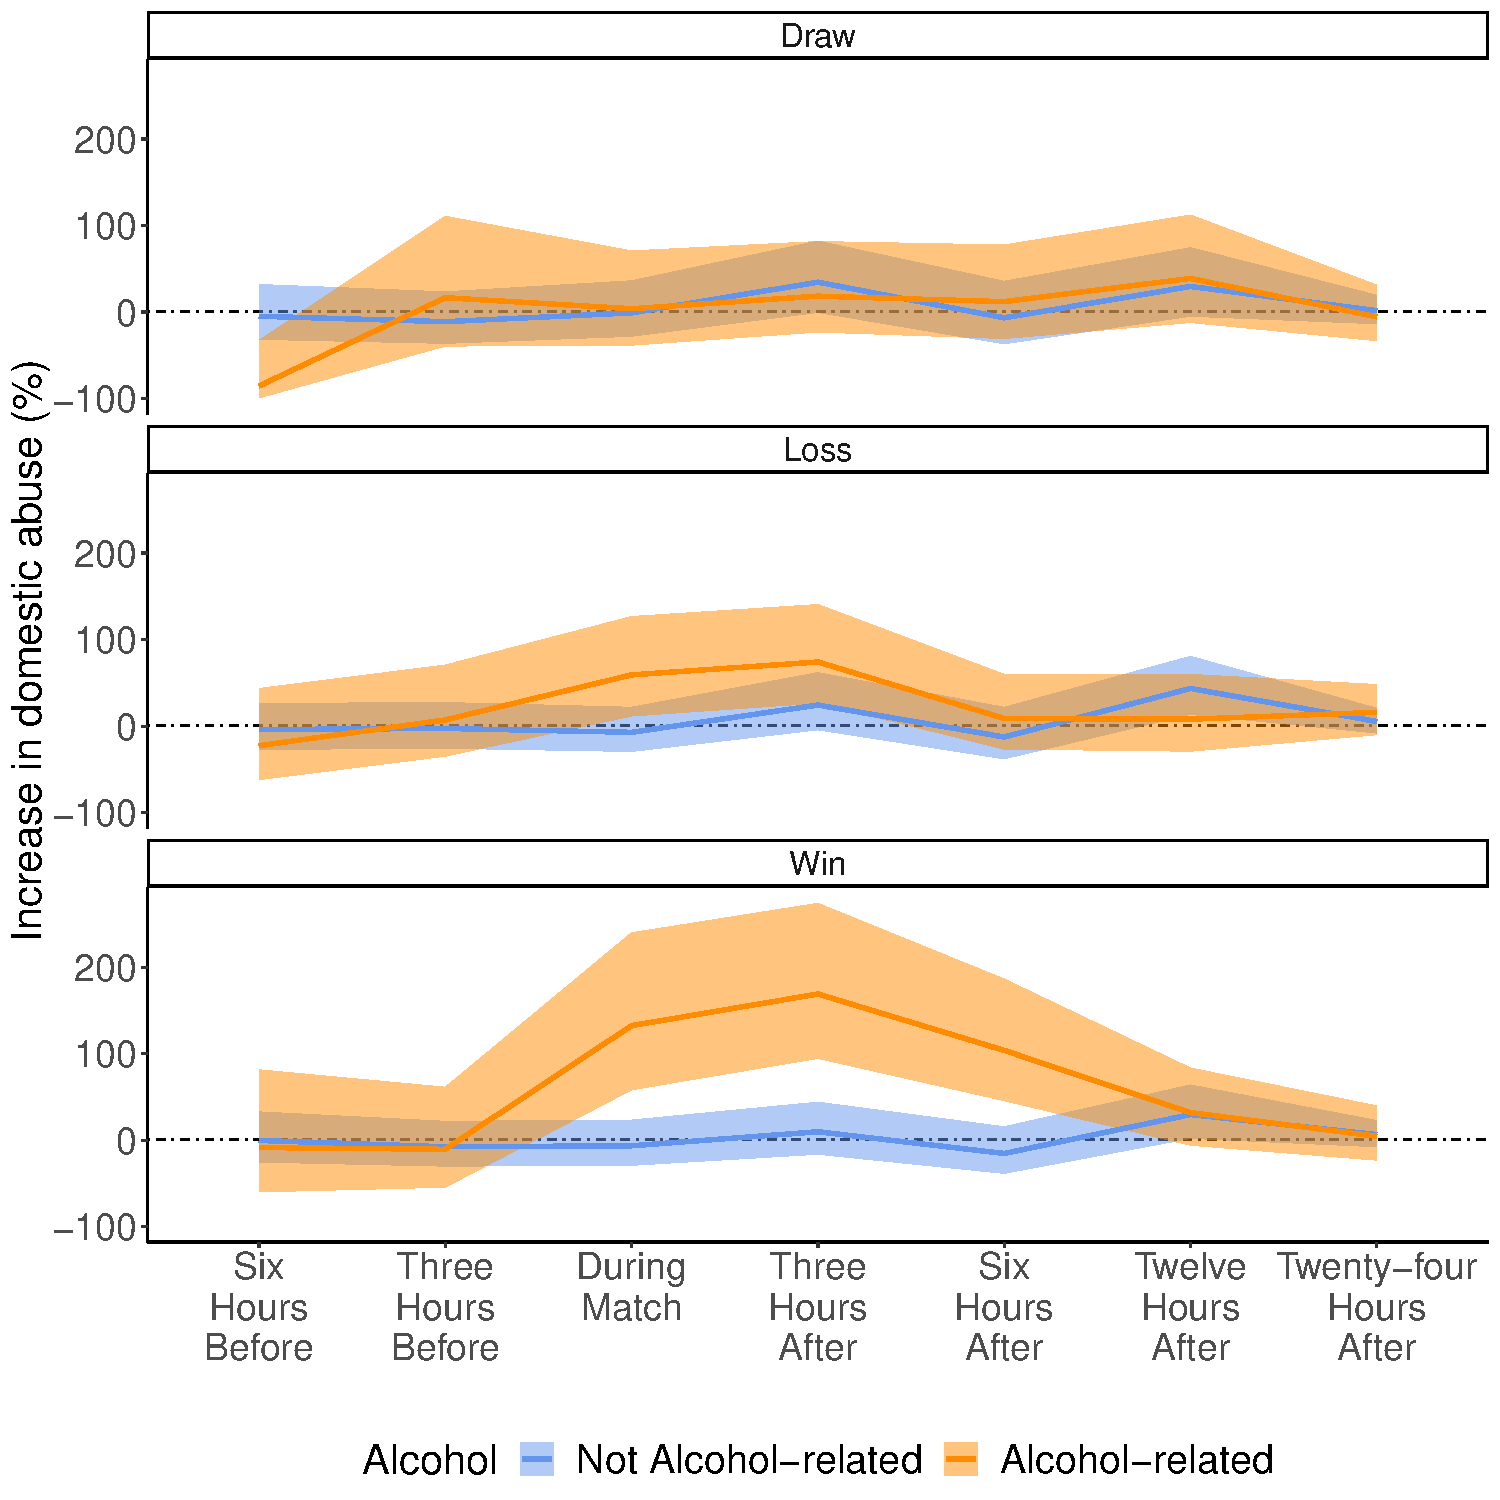
\includegraphics[width=0.45\textwidth]{Threehours.pdf}
\label{fig:threehours}
\caption*{Note: Estimates are from two separate negative binomial regressions (based on tests of overdispersion) with year, month, day of week, three-hour period of day, Christmas, New Year's eve controls. Shaded area is 95\% CIs.}
\end{figure}

\newpage

\section*{Discussion}

Our results have shown that an England victory in a national football tournament is followed by a 61\% increase in the reported number of alcohol-related domestic abuse cases. This is a large effect, translating into a 0.43 increase in the daily rate of alcohol-related cases per 100,000 individuals, against a base rate 0.71 cases per 100,000. The effect is entirely limited to alcohol-related abuse, even though alcohol-related domestic abuse cases comprise only 23\% of all domestic abuse in our dataset. As such, we see this as strong quantitative evidence that alcohol plays an instrumental role in the relationship between football and domestic abuse in England. The effect is also exclusively limited to male-perpetrated domestic abuse, implicating masculinity and alcohol consumption as the pathway by which football increases abuse. The temporal pattern of the increase following an England victory is highly consistent with a causal explanation, further supported by the fact that the allocation of England win days can be considered random. %\AT{Is this ok?} \TM{I really like this paragraph}


Our findings show both similarities and differences with results from previous quantitative investigations. Replicating the results of a previous US study, we found that it is male to female abuse that is affected by a sporting event \cite{Card2011}. In the same study, the effect of the match did not depend on alcohol-involvement in the abuse case, and the increase was driven by unexpected losses. In contrast, we find that in the context of England and football, it is a victory that results in the largest increase, and that alcohol involvement is critical. This discrepancy most likely stems from the contextual differences between the two studies (England, football, national tournaments vs. US, American football, NFL matches), highlighting that the effect of sports-induced emotional cues on domestic abuse is highly sensitive to the cultural context. 

Based on the pre-match betting odds, all of the England victories were expected in our dataset. This suggests that in the context of England's participation in national football tournaments, it is living up to the expectations of the fans that results in largest emotional effect. Indeed, English newspapers' narratives about the team's performance in these tournaments are characterised with high levels of optimism, expectation and yearning for the glory of the 1966 World Cup \cite{Vincent2010}. Previous research has demonstrated how the vicarious experience of watching their team play can increase supporter's testosterone and cortisol levels, even when they expect their team to win, suggested to be an adaptive response to the perceived threat to one's social identity \cite{VanderMeij2012}. Anecdotal evidence suggests that alcohol consumption increases following an England victory \cite{Davies2018}, consistent with our findings.


The most widely-discussed England-based investigation of the link between football and domestic abuse \cite{Kirby2014} have found that an England loss results in the most pronounced increase in domestic abuse (38\%), and a win or draw have a slightly smaller effect (26\%). This study used daily data on IPV from Lancashire Constabulary (serving a population of 1.4 million, about half the population of the West Midlands) for the period of the 2002, 2004 and 2010 World Cup tournaments (June-July). 
Using daily domestic abuse data from the West Midlands for the period between 2010 and 2018, we find a different pattern, with the largest increase in alcohol-involved cases of abuse when England wins, but no comparable effects when England loses. Upon re-analysing their data by treating wins and draws as two separate variables (resulting in an improved model fit, see Table \ref{kirbyrep1} in SI Appendix), we see a roughly similar effect for wins (45\%, 95\% CI [28\%--64\%]) and losses (39\%, 95\% CI [18\%--64\%]), and no effect when England draws. Our reanalysis replicates the win effect seen in the current data in the earlier sample, though the absence of a loss effect remains a stark difference between the two studies. While our sample sizes are different (92 days versus 3,017 days), and our respective samples cover different geographical areas and time periods, the discrepancy is still puzzling. 


To explore the underlying reason for this discrepancy and test the robustness of our results, we find it instructive to break our analysis into specific tournament years for the two datasets (see Table \ref{kirbyrep2} in SI Appendix). An interesting common pattern in both datasets is the large effect of England's victory over Slovenia in the group stage of the 2010 World Cup, which, after much anticipation, secured their progression to the next stage of the tournament. Equally, the subsequent loss against Germany in the knockout stage resulted in a substantial increase in the number of reported domestic abuse incidents, which is the only tournament in our dataset where this pattern appears. Interestingly, an earlier examination of the 2010 World Cup found a similar pattern, using daily data from 33 out of 39 police forces in England\cite{Brimicombe2012}, although our much larger sample size (3,017 days versus 62 days) allows for a more precise assessment of the link between football and domestic abuse.


While the effect of a victory or loss is likely to be highly specific to the context of a particular match (e.g., group stage or knockout stage, previous performance of the team, weather on the day, etc.), the estimated effect of an England victory on the number of reported domestic abuse cases is robust to different model specifications (see Table \ref{specifications}), using data from a different geographical area (see Table \ref{kirbyrep2} in SI Appendix), and the exclusion of specific tournament years (see Table \ref{robustness} in SI Appendix). 

Does this effect generalise to other sporting events, or is it specific to football?
It has been previously suggested that other popular sports, such as rugby have similar links with domestic abuse \cite{Brooks-Hay2018}. Rugby is the second most popular sport in England after football \cite{Ipsos2003}. Focusing on the Six Nations, a high-profile rugby tournament that takes place every year with the participation of England, Wales, Scotland, Ireland, France and Italy, we explored whether the reported number of domestic abuse cases increase on days when the England national rugby team plays. Between 2010 and 2018, there are many more win and loss days of the England rugby union team compared to the England national football team. The results show no comparable effects for rugby matches (see Table \ref{rugby} in SI Appendix), potentially stemming from differences in media coverage, audience numbers, and the role of alcohol between the two tournaments. 
%\TM{And possibly the differnt role of alcohol within the culture of the two sports?}

We also investigated whether England match days have similar effects on other types of non-domestic abusive behaviours, including sexual offences, child and vulnerable adult abuse. A commonality between domestic abuse and these types of offences is the element of control and domination, although domestic abuse is much more frequent in our dataset. We find no evidence that England matches have comparable effects on non-domestic sexual offences and other abuse cases (see Table \ref{otherabuse} in SI Appendix). 

Our data further allows us to explore the characteristics of alcohol-related domestic abuse perpetrated on England match days. First, using a series of logistic regressions, we investigate whether these cases are more likely to be newly reported (with no earlier record for the same victim-offender pair in our dataset), happen in a residential dwelling as opposed to a public location, or result in an injury. We find no evidence that domestic abuse cases perpetrated on England match days are more likely to be newly reported (see Table \ref{Characteristics1} in SI Appendix), compared to domestic abuse cases occurring on non-match days. It could be argued that since fans often congregate in pubs to watch England play, there is a higher likelihood that domestic abuse occurs in public and get reported on these days. Interestingly, our results indicate that, compared to non-match days, reported cases are more likely to be perpetrated in public on England loss days, but not on England win days, and that this effect does not differ by alcohol-involvement in the case. Non-alcohol related cases reported on England loss days are also more likely to result in an injury, a pattern that is absent from alcohol-related cases.

Next, we turn to repeated cases of domestic abuse (multiple cases with the same victim-offender pair). Domestic abuse is rarely a one-off incident, and reported repeat cases allow us to explore the characteristics of domestic abuse that occurs on match days in more detail. We are interested in whether the number of days elapsed between two consecutive cases is affected by England football matches. For example, it is possible that England match days bring reported cases of domestic abuse forward, which would have otherwise happened at a later point in time. We investigate this question with two negative binomial regressions, where the outcome variables are the number of days elapsed since the last reported case, and the number of days until the next case, respectively. In addition, using all reported cases, we explore whether the number of hours elapsed before reporting the case is affected by England match days.


The results show that non-alcohol related cases perpetrated on England loss days occur fewer days after the previous incident, 192 days, 95\% CI [159 days, 232 days], compared to non-alcohol repeat cases reoccurring on non-match days, 226 days, 95\% CI [207 days, 248 days] (see Table \ref{Characteristics2} in SI Appendix). Non-alcohol related domestic abuse cases perpetrated on England win days are more likely to be followed by another case of abuse in fewer days, 172 days, 95\% CI [138 days, 214 days], compared to cases occurring on non-match days, 242 days, 95\% CI [223 days, 261 days], and this pattern is absent from alcohol-related cases. Interestingly, non-alcohol related cases perpetrated on England loss days are likely to be reported after fewer hours, 59 hours, 95\% CI [45 hours, 78 hours], compared to non-alcohol related abuse perpetrated on non-match days, 104 hours, 95\% CI [91 hours, 119 hours]. 

%The results show that non-alcohol related cases perpetrated on England loss days occur slightly sooner after the previous incident, compared to non-alcohol cases reoccurring on non-match days (see Table \ref{Characteristics2} in the Appendix). Non-alcohol related domestic abuse cases perpetrated on England win days or the day after an England match are more likely to be followed by another case of abuse sooner, compared to non-alcohol cases occurring on non-match days. Interestingly, non-alcohol related cases perpetrated on England loss days or on days following an England match day are likely to be reported sooner, compared to non-alcohol related abuse perpetrated on non-match days. 

It is perhaps surprising that while we found no evidence for an increase in the reported number of domestic abuse cases on England loss days (see Table \ref{specifications}), domestic abuse perpetrated on these days seems to be characteristically different from domestic abuse perpetrated on other days. More specifically, cases perpetrated on England loss days are more likely to occur outside, result in an injury, and get reported sooner. Furthermore, repeated cases perpetrated on England loss days occur slightly sooner following the previous case, but abuse perpetrated on England win days are followed by another incident sooner. While these findings should be interpreted with caution due to the pervasive problem of underreporting, the results suggest differences in the effect of England wins and losses on domestic abuse. In particular, while there is no increase in the overall number of cases reported on England loss days, incidents reported on these days are characteristically different from abuse perpetrated on non-match days, while we observe a substantial difference in the number, but not the characteristics of cases perpetrated on England win days.



%Note: please start your introduction without including the word ``Introduction'' as a section heading (except for math articles in the Physical Sciences section); this heading is implied in the first paragraphs. 

%\section*{Guide to using this template on Overleaf}

%Please note that whilst this template provides a preview of the typeset manuscript for submission, to help in this preparation, it will not necessarily be the final publication layout. For more detailed information please see the \href{http://www.pnas.org/site/authors/format.xhtml}{PNAS Information for Authors}.

%If you have a question while using this template on Overleaf, please use the help menu (``?'') on the top bar to search for \href{https://www.overleaf.com/help}{help and tutorials}. You can also \href{https://www.overleaf.com/contact}{contact the Overleaf support team} at any time with specific questions about your manuscript or feedback on the template.

%\subsection*{Author Affiliations}

%Include department, institution, and complete address, with the ZIP/postal code, for each author. Use lower case letters to match authors with institutions, as shown in the example. Authors with an ORCID ID may supply this information at submission.

%\subsection*{Submitting Manuscripts}

%All authors must submit their articles at \href{http://www.pnascentral.org/cgi-bin/main.plex}{PNAScentral}. If you are using Overleaf to write your article, you can use the ``Submit to PNAS'' option in the top bar of the editor window. 

%\subsection*{Format}

%Many authors find it useful to organize their manuscripts with the following order of sections;  Title, Author Affiliation, Keywords, Abstract, Significance Statement, Results, Discussion, Materials and methods, Acknowledgments, and References. Other orders and headings are permitted.

%\subsection*{Manuscript Length}
%
%PNAS generally uses a two-column format averaging 67 characters, including spaces, per line. The maximum length of a Direct Submission research article is six pages and a Direct Submission Plus research article is ten pages including all text, spaces, and the number of characters displaced by figures, tables, and equations.  When submitting tables, figures, and/or equations in addition to text, keep the text for your manuscript under 39,000 characters (including spaces) for Direct Submissions and 72,000 characters (including spaces) for Direct Submission Plus.
%
%\subsection*{References}
%
%References should be cited in numerical order as they appear in text; this will be done automatically via bibtex, e.g. \cite{belkin2002using} and \cite{berard1994embedding,coifman2005geometric}. All references should be included in the main manuscript file.  
%
%\subsection*{Data Archival}
%
%PNAS must be able to archive the data essential to a published article. Where such archiving is not possible, deposition of data in public databases, such as GenBank, ArrayExpress, Protein Data Bank, Unidata, and others outlined in the Information for Authors, is acceptable.
%
%\subsection*{Language-Editing Services}
%Prior to submission, authors who believe their manuscripts would benefit from professional editing are encouraged to use a language-editing service (see list at www.pnas.org/site/authors/language-editing.xhtml). PNAS does not take responsibility for or endorse these services, and their use has no bearing on acceptance of a manuscript for publication. 
%
%\begin{figure}%[tbhp]
%\centering
%
\includegraphics[width=.8\linewidth]{frog}
%\caption{Placeholder image of a frog with a long example caption to show justification setting.}
%\label{fig:frog}
%\end{figure}
%
%
%\begin{SCfigure*}[\sidecaptionrelwidth][t]
%\centering
%
\includegraphics[width=11.4cm,height=11.4cm]{frog}
%\caption{This caption would be placed at the side of the figure, rather than below it.}\label{fig:side}
%\end{SCfigure*}
%
%\subsection*{Digital Figures}
%
%Only TIFF, EPS, and high-resolution PDF for Mac or PC are allowed for figures that will appear in the main text, and images must be final size. Authors may submit U3D or PRC files for 3D images; these must be accompanied by 2D representations in TIFF, EPS, or high-resolution PDF format.  Color images must be in RGB (red, green, blue) mode. Include the font files for any text. 
%
%Figures and Tables should be labelled and referenced in the standard way using the \verb|\label{}| and \verb|\ref{}| commands.
%
%Figure \ref{fig:frog} shows an example of how to insert a column-wide figure. To insert a figure wider than one column, please use the \verb|\begin{figure*}...\end{figure*}| environment. Figures wider than one column should be sized to 11.4 cm or 17.8 cm wide. Use \verb|\begin{SCfigure*}...\end{SCfigure*}| for a wide figure with side captions.
%
%\subsection*{Tables}
%In addition to including your tables within this manuscript file, PNAS requires that each table be uploaded to the submission separately as a “Table” file.  Please ensure that each table .tex file contains a preamble, the \verb|\begin{document}| command, and the \verb|\end{document}| command. This is necessary so that the submission system can convert each file to PDF.
%
%\subsection*{Single column equations}
%
%Authors may use 1- or 2-column equations in their article, according to their preference.
%
%To allow an equation to span both columns, use the \verb|\begin{figure*}...\end{figure*}| environment mentioned above for figures.
%
%Note that the use of the \verb|widetext| environment for equations is not recommended, and should not be used. 
%
%\begin{figure*}[bt!]
%\begin{align*}
%(x+y)^3&=(x+y)(x+y)^2\\
%       &=(x+y)(x^2+2xy+y^2) \numberthis \label{eqn:example} \\
%       &=x^3+3x^2y+3xy^3+x^3. 
%\end{align*}
%\end{figure*}
%
%
%\begin{table}%[tbhp]
%\centering
%\caption{Comparison of the fitted potential energy surfaces and ab initio benchmark electronic energy calculations}
%\begin{tabular}{lrrr}
%Species & CBS & CV & G3 \\
%\midrule
%1. Acetaldehyde & 0.0 & 0.0 & 0.0 \\
%2. Vinyl alcohol & 9.1 & 9.6 & 13.5 \\
%3. Hydroxyethylidene & 50.8 & 51.2 & 54.0\\
%\bottomrule
%\end{tabular}
%
%\addtabletext{nomenclature for the TSs refers to the numbered species in the table.}
%\end{table}

%
%Authors should submit SI as a single separate PDF file, combining all text, figures, tables, movie legends, and SI references.  PNAS will publish SI uncomposed, as the authors have provided it.  Additional details can be found here: \href{http://www.pnas.org/page/authors/journal-policies}{policy on SI}.  For SI formatting instructions click \href{https://www.pnascentral.org/cgi-bin/main.plex?form_type=display_auth_si_instructions}{here}.  The PNAS Overleaf SI template can be found \href{https://www.overleaf.com/latex/templates/pnas-template-for-supplementary-information/wqfsfqwyjtsd}{here}.  Refer to the SI Appendix in the manuscript at an appropriate point in the text. Number supporting figures and tables starting with S1, S2, etc.
%
%Authors who place detailed materials and methods in an SI Appendix must provide sufficient detail in the main text methods to enable a reader to follow the logic of the procedures and results and also must reference the SI methods. If a paper is fundamentally a study of a new method or technique, then the methods must be described completely in the main text.
%
%\subsubsection*{SI Datasets} 
%
%Supply Excel (.xls), RTF, or PDF files. This file type will be published in raw format and will not be edited or composed.
%
%
%\subsubsection*{SI Movies}
%
%Supply Audio Video Interleave (avi), Quicktime (mov), Windows Media (wmv), animated GIF (gif), or MPEG files and submit a brief legend for each movie in a Word or RTF file. All movies should be submitted at the desired reproduction size and length. Movies should be no more than 10 MB in size.
%
%
%\subsubsection*{3D Figures}
%
%Supply a composable U3D or PRC file so that it may be edited and composed. Authors may submit a PDF file but please note it will be published in raw format and will not be edited or composed.


\matmethods{
Our dataset comprises all crimes and specific types of incidents (such as domestic abuse) that have been reported to the West Midlands Police (the third largest police force in England \cite{Homeoffice}, serving an estimated 2.9 million people in 2017, \citenum{populationfigure}) in the period between 2010 and 2018. The first half of 2017 has been excluded due to missing data. The number of reported domestic abuse cases is the sum of crimes that have a domestic abuse marker, and all domestic abuse incidents. Crimes that have a domestic abuse marker indicate cases of domestic abuse that meet the criteria for notifiable offences in the UK, whereas domestic abuse incidents refer to cases that do not qualify as a crime. For each record in this dataset, we have information about the time and location of the incident or crime, and the gender and age of the offender and victim. We restricted our analyses to cases with one victim and one offender. We can also identify repeat offenders and victims by their unique person identifier. Domestic abuse cases comprise about 31\% of all recorded crimes and incidents in the dataset, and about 23\% of all domestic abuse cases are alcohol-related. In the period between 2010 and 2018, the daily rate of non-alcohol related domestic incidents falls between 1.6-3 cases per 100,000 individuals, whereas the daily rate of alcohol-related cases falls between 0.35-1 cases per 100,000 individuals. There were three World Cups (2010, 2014, 2018) and two European Championships (2012, 2016) in the period covered by our dataset. All included tournaments took place in the months of June and July.

 To analyse the temporal dynamics of the England win effect (see Figure \ref{fig:threehours}), we divided each day in our dataset into eight three-hour periods, the first one starting at 12am, and used these to identify specific time windows around the time of the match. The exact time of the matches vary considerably (the earliest starting at 1pm, and the latest at 11pm). We first identified the three-hour period of the day into which each match falls. If the start and end time of the match did not fall in the same three-hour period, we chose the three-hour period that covers the larger part of the match (e.g., a 2.5 hour long match starting at 7pm will be assigned to the 6-9pm period and not to the 9pm-12am period).

}

\showmatmethods{} % Display the Materials and Methods section


%\acknow{Please include your acknowledgments here, set in a single paragraph. Please do not include any acknowledgments in the Supporting Information, or anywhere else in the manuscript.}

%\showacknow{} % Display the acknowledgments section

% Bibliography
\bibliography{football_refs}


\clearpage

\section*{Supporting Information (SI)}

\renewcommand{\thetable}{S\arabic{table}}
\renewcommand{\thefigure}{S\arabic{figure}}
\setcounter{table}{0}
\setcounter{figure}{0}

\begin{table}[!ht]
\centering
 \caption{Non-domestic violent cases by gender}
  \label{otherviolence_gender}
 \scalebox{0.9}{
   \begin{threeparttable}
\begin{tabular}{@{\extracolsep{5pt}}lcccc} 
\\[-1.8ex]\hline 
\hline \\[-1.8ex] 
 & \multicolumn{4}{c}{\textit{Dependent variable:}} \\ 
\cline{2-5} 
\\[-1.8ex] & \multicolumn{4}{c}{Number of other violent abuse cases per day} \\ 
\\
 & Male & Male & Female & Female \\ 
 & to Male & to Female & to Female & to Male \\ 
\\[-1.8ex] & (1) & (2) & (3) & (4)\\ 
\hline \\[-1.8ex] 
% Alcohol & $-$0.900$^{***}$ & $-$0.891$^{***}$ & $-$0.864$^{***}$ & $-$0.921$^{***}$ \\ 
%  & (0.048) & (0.033) & (0.080) & (0.066) \\ 
  Tournament on & 0.037 & 0.050$^{**}$ & 0.041 & 0.051 \\ 
  & (0.026) & (0.021) & (0.038) & (0.036) \\ 
  England win & 0.013 & 0.019 & $-$0.031 & 0.174 \\ 
  & (0.082) & (0.067) & (0.111) & (0.112) \\ 
  England draw & 0.089 & 0.012 & 0.115 & 0.042 \\ 
  & (0.094) & (0.078) & (0.139) & (0.132) \\ 
  England loss & 0.018 & 0.028 & 0.088 & 0.118 \\ 
  & (0.082) & (0.066) & (0.114) & (0.108) \\ 
  After England & 0.085 & 0.070 & 0.181$^{**}$ & 0.149$^{**}$ \\ 
  & (0.050) & (0.042) & (0.071) & (0.067) \\ 
  Alcohol:Tournament on & $-$0.027 & $-$0.086$^{**}$ & $-$0.077 & $-$0.167$^{**}$ \\ 
  & (0.055) & (0.038) & (0.087) & (0.073) \\ 
  Alcohol:England win & 0.391$^{**}$ & 0.613$^{***}$ & 0.441$^{*}$ & $-$0.114 \\ 
  & (0.158) & (0.109) & (0.251) & (0.199) \\ 
  Alcohol:England draw & 0.071 & 0.102 & 0.127 & $-$0.337 \\ 
  & (0.192) & (0.137) & (0.361) & (0.254) \\ 
  Alcohol:England loss & 0.296$^{*}$ & 0.057 & $-$0.023 & 0.027 \\ 
  & (0.153) & (0.112) & (0.237) & (0.207) \\ 
  Alcohol:After England & 0.208$^{*}$ & 0.053 & $-$0.119 & $-$0.158 \\ 
  & (0.100) & (0.072) & (0.163) & (0.136) \\ 
 \hline \\[-1.8ex] 
Number of days & 3,017 & 3,017 & 3,017 & 3,017 \\ 
%Log Likelihood & $-$17,204.240 & $-$21,360.820 & $-$13,708.300 & $-$14,378.320 \\ 
%$\theta$ & 44.231$^{***}$  (2.800) & 43.449$^{***}$  (1.546) & 24.998$^{***}$  (1.919) & 35.978$^{***}$  (3.376) \\ 
%Akaike Inf. Crit. & 34,540.480 & 42,853.640 & 27,548.590 & 28,888.630 \\ 
\hline 
\hline \\[-1.8ex] 
%\textit{Note:}  & \multicolumn{4}{r}{$^{*}$p$<$0.1; $^{**}$p$<$0.05; $^{***}$p$<$0.01} \\ 
\end{tabular} 
\begin{tablenotes}
     \item[a] \textit{$^{*}$p$<$0.1; $^{**}$p$<$0.05; $^{***}$p$<$0.01}
      \item[b] \textit{Estimates are from a series of negative binomial regressions (based on tests of overdispersion)  with year, month, day of week, Christmas, New Year's eve controls interacted with alcohol; standard errors in parentheses}
    \end{tablenotes}
\end{threeparttable} }
\end{table}

\newpage

\begin{table}[htp]
\centering
 \caption{Replication of Kirby et al. (2014) with an alternative specification}
   \label{kirbyrep1}
 \begin{threeparttable}
\begin{tabular}{@{\extracolsep{5pt}}lcc} 
\\[-1.8ex]\hline 
\hline \\[-1.8ex] 
 & \multicolumn{2}{c}{\textit{Dependent variable:}} \\ 
\cline{2-3} 
\\[-1.8ex] & \multicolumn{2}{c}{Number of reported IPV cases per day} \\ 
\\ 
 & Original Model & Win/Draw Separate \\ 
\\[-1.8ex] & (1) & (2)\\ 
\hline \\[-1.8ex] 
 England windraw & 0.256$^{***}$ &  \\ 
  & (0.055) &  \\ 
  England win &  & 0.452$^{***}$ \\ 
  &  & (0.064) \\ 
  England draw &  & 0.032 \\ 
  &  & (0.073) \\ 
  England loss & 0.382$^{***}$ & 0.388$^{***}$ \\ 
  & (0.094) & (0.085) \\ 
  After England & 0.111$^{**}$ & 0.113$^{**}$ \\ 
  & (0.051) & (0.047) \\ 
 \hline \\[-1.8ex] 
Number of days & 92 & 92 \\ 
AIC & 714.980 & 704.356 \\ 
%BIC & 747.763 & 739.662 \\ 
%\hline 
\hline \\[-1.8ex] 
%\textit{Note:}  & \multicolumn{2}{r}{$^{*}$p$<$0.1; $^{**}$p$<$0.05; $^{***}$p$<$0.01} \\ 
\end{tabular} 
\begin{tablenotes}
      \item[a] \textit{$^{*}$p$<$0.1; $^{**}$p$<$0.05; $^{***}$p$<$0.01}
      \item[b] \textit{Estimates are from a series of negative binomial regressions (based on tests of overdispersion) with year and day of week controls; standard errors in parentheses; data is only available during the tournament period}
    \end{tablenotes}
\end{threeparttable} 
\end{table}

\newpage

\begin{sidewaystable}[htp]
\centering
 \caption{Year subgroup regressions, Lancashire and West Midlands data}
   \label{kirbyrep2}
    \scalebox{0.78}{
 \begin{threeparttable}
\begin{tabular}{@{\extracolsep{5pt}}lcccccccc} 
\\[-1.8ex]\hline 
\hline \\[-1.8ex] 
 & \multicolumn{8}{c}{\textit{Dependent variable:}} \\ 
\cline{2-9} 
\\[-1.8ex] & \multicolumn{3}{c}{Number of IPV cases per day in Lancashire} & \multicolumn{5}{c}{Number of domestic abuse cases per day in West Midlands} \\ 
\\[-1.8ex] & \textit{negative} & \multicolumn{2}{c}{\textit{Poisson}} & \multicolumn{5}{c}{\textit{negative}} \\ 
 & \textit{binomial} & \multicolumn{2}{c}{\textit{}} & \multicolumn{5}{c}{\textit{binomial}} \\ 
 & 2002 & 2006 & 2010 & 2010 & 2012 & 2014 & 2016 & 2018 \\ 
\\[-1.8ex] & (1) & (2) & (3) & (4) & (5) & (6) & (7) & (8)\\ 
\hline \\[-1.8ex] 
 Tournament on &  &  &  & 0.074$^{*}$ & $-$0.066 & $-$0.048 & 0.035 & 0.089$^{*}$ \\ 
  &  &  &  & (0.041) & (0.085) & (0.044) & (0.041) & (0.044) \\ 
  England win & 0.596$^{***}$ & 0.297$^{***}$ & 0.916$^{***}$ & 0.050 & $-$0.237 &  & $-$0.008 & 0.061 \\ 
  & (0.152) & (0.077) & (0.114) & (0.155) & (0.175) &  & (0.151) & (0.077) \\ 
  England draw & 0.100 & 0.098 & $-$0.137 & $-$0.029 & 0.324 & $-$0.077 & $-$0.021 &  \\ 
  & (0.150) & (0.156) & (0.095) & (0.112) & (0.204) & (0.173) & (0.108) &  \\ 
  England loss & 0.200 & 0.373$^{***}$ & 0.568$^{***}$ & 0.174 & $-$0.127 & $-$0.042 & $-$0.155 & 0.066 \\ 
  & (0.232) & (0.117) & (0.106) & (0.140) & (0.212) & (0.124) & (0.154) & (0.088) \\ 
  After England & 0.253$^{**}$ & 0.122$^{*}$ & 0.024 & 0.070 & $-$0.008 & 0.007 & 0.038 & 0.140$^{**}$ \\ 
  & (0.101) & (0.070) & (0.065) & (0.082) & (0.125) & (0.103) & (0.081) & (0.060) \\ 
%  AlcoholYes &  &  &  & $-$0.853$^{***}$ & $-$0.803$^{***}$ & $-$0.704$^{***}$ & $-$0.725$^{***}$ & $-$0.743$^{***}$ \\ 
%  &  &  &  & (0.083) & (0.097) & (0.067) & (0.059) & (0.062) \\ 
  Tournament on:Alcohol &  &  &  & $-$0.093 & 0.076 & 0.063 & $-$0.163$^{**}$ & $-$0.068 \\ 
  &  &  &  & (0.101) & (0.162) & (0.076) & (0.072) & (0.078) \\ 
  England win:Alcohol &  &  &  & 2.558$^{***}$ & 0.756$^{*}$ &  & 0.348 & 0.460$^{***}$ \\ 
  &  &  &  & (0.277) & (0.314) &  & (0.257) & (0.123) \\ 
  England draw:Alcohol &  &  &  & 0.078 & $-$0.581 & 0.089 & 0.129 &  \\ 
  &  &  &  & (0.246) & (0.571) & (0.307) & (0.180) &  \\ 
  England loss:Alcohol &  &  &  & 0.748$^{**}$ & 0.301 & 0.048 & $-$0.289 & 0.160 \\ 
  &  &  &  & (0.259) & (0.372) & (0.206) & (0.322) & (0.149) \\ 
  After England:Alcohol &  &  &  & 0.128 & $-$0.072 & 0.068 & $-$0.112 & 0.188$^{*}$ \\ 
  &  &  &  & (0.183) & (0.254) & (0.171) & (0.144) & (0.102) \\ 
 \hline \\[-1.8ex] 
Number of days & 30 & 32 & 30 & 730 & 732 & 730 & 732 & 618 \\ 
%Log Likelihood & $-$112.494 & $-$101.847 & $-$107.268 & $-$2,315.879 & $-$2,259.612 & $-$2,604.474 & $-$2,614.295 & $-$2,237.868 \\ 
%$\theta$ & 57.581$^{*}$  (31.978) &  &  & 136.319$^{***}$  (31.759) & 55.994$^{***}$  (9.013) & 68.164$^{***}$  (8.225) & 109.262$^{***}$  (16.375) & 90.905$^{***}$  (12.959) \\ 
%Akaike Inf. Crit. & 246.989 & 225.694 & 236.536 & 4,731.757 & 4,619.224 & 5,304.947 & 5,328.590 & 4,563.737 \\ 
\hline 
\hline \\[-1.8ex] 
%\textit{Note:}  & \multicolumn{8}{r}{$^{*}$p$<$0.1; $^{**}$p$<$0.05; $^{***}$p$<$0.01} \\ 
\end{tabular} 
\begin{tablenotes}
      \item[a] \textit{$^{*}$p$<$0.1; $^{**}$p$<$0.05; $^{***}$p$<$0.01}
      \item[b] \textit{Estimates are from a series of negative binomial  or poisson regressions (based on tests of overdispersion). The first three regressions have day of week control, the rest of the regressions have month, day of week, Christmas, New Year's eve controls interacted with alcohol; standard errors in parentheses}
    \end{tablenotes}
\end{threeparttable} }
\end{sidewaystable}

\newpage



\begin{table}[htp]
\centering
 \caption{Robustness of the result: sensitivity to the exclusion of specific years}
  \label{robustness}
 \scalebox{0.7}{
  \begin{threeparttable}
\begin{tabular}{@{\extracolsep{5pt}}lccccc} 
\\[-1.8ex]\hline 
\hline \\[-1.8ex] 
 & \multicolumn{5}{c}{\textit{Dependent variable:}} \\ 
 \cline{2-6} 
\\[-1.8ex] 
  & \multicolumn{5}{c}{Number of domestic abuse cases per day} \\ 
 \\
%\\[-1.8ex] & \multicolumn{5}{c}{N} \\ 
 & 2018 & 2016 & 2014 & 2012 & 2010 \\ 
  &  excluded & excluded & excluded & excluded & excluded \\ 
\\[-1.8ex] & (1) & (2) & (3) & (4) & (5)\\ 
\hline \\[-1.8ex] 
%Alcohol & $-$0.862$^{***}$ & $-$0.862$^{***}$ & $-$0.862$^{***}$ & $-$0.863$^{***}$ & $-$0.867$^{***}$ \\ 
  & (0.033) & (0.033) & (0.032) & (0.031) & (0.033) \\ 
  Tournament on & 0.018 & 0.015 & 0.027 & 0.030 & $-$0.003 \\ 
  & (0.022) & (0.025) & (0.025) & (0.022) & (0.025) \\ 
  England win & $-$0.093 & $-$0.047 & $-$0.029 & 0.019 & $-$0.051 \\ 
  & (0.097) & (0.068) & (0.062) & (0.066) & (0.067) \\ 
  England draw & 0.038 & 0.077 & 0.057 & 0.004 & 0.046 \\ 
  & (0.072) & (0.091) & (0.078) & (0.075) & (0.088) \\ 
  England loss & 0.030 & 0.066 & 0.053 & 0.054 & 0.013 \\ 
  & (0.079) & (0.065) & (0.069) & (0.062) & (0.065) \\ 
  After England & 0.057 & 0.080$^{*}$ & 0.088$^{**}$ & 0.099$^{**}$ & 0.071$^{*}$ \\ 
  & (0.048) & (0.042) & (0.040) & (0.039) & (0.042) \\ 
  Alcohol:Tournament on & $-$0.086$^{**}$ & $-$0.037 & $-$0.118$^{***}$ & $-$0.092$^{**}$ & $-$0.048 \\ 
  & (0.039) & (0.046) & (0.047) & (0.040) & (0.042) \\ 
  Alcohol:England win & 0.884$^{***}$ & 0.674$^{***}$ & 0.609$^{***}$ & 0.574$^{***}$ & 0.511$^{***}$ \\ 
  & (0.163) & (0.109) & (0.100) & (0.105) & (0.107) \\ 
  Alcohol:England draw & $-$0.046 & $-$0.141 & $-$0.048 & 0.055 & $-$0.017 \\ 
  & (0.130) & (0.179) & (0.141) & (0.131) & (0.151) \\ 
  Alcohol:England loss & 0.014 & 0.139 & 0.131 & 0.078 & 0.039 \\ 
  & (0.134) & (0.107) & (0.116) & (0.103) & (0.109) \\ 
  Alcohol:After England & $-$0.065 & 0.096 & 0.050 & 0.054 & 0.050 \\ 
  & (0.086) & (0.073) & (0.071) & (0.067) & (0.071) \\ 
 \hline \\[-1.8ex] 
Number of days & 2,708 & 2,651 & 2,652 & 2,651 & 2,652 \\ 
%Log Likelihood & $-$18,626.890 & $-$18,243.850 & $-$18,269.330 & $-$18,506.890 & $-$18,533.610 \\ 
%$\theta$ & 60.431$^{***}$  (2.862) & 58.624$^{***}$  (2.761) & 62.319$^{***}$  (3.016) & 67.975$^{***}$  (3.245) & 59.902$^{***}$  (2.752) \\ 
%Akaike Inf. Crit. & 37,381.780 & 36,615.700 & 36,666.660 & 37,141.780 & 37,195.210 \\ 
\hline 
%\hline \\[-1.8ex] 
%\textit{Note:}  & \multicolumn{6}{r}{$^{*}$p$<$0.1; $^{**}$p$<$0.05; $^{***}$p$<$0.01} \\ 
%\end{tabular} 
%\end{table} 

\end{tabular}
\begin{tablenotes}
      \item[a] \textit{$^{*}$p$<$0.1; $^{**}$p$<$0.05; $^{***}$p$<$0.01}
      \item[b] \textit{Estimates are from a series of negative binomial regressions (based on tests of overdispersion)  with year, month, day of week, Christmas, New Year's eve controls interacted by alcohol; standard errors in parentheses}
    \end{tablenotes}
\end{threeparttable} } 
\end{table}

\newpage

\begin{table}[htp]
\centering
 \scalebox{0.85}{
  \begin{threeparttable}
 \caption{The effect of England matches in the Six Nations rugby tournament on domestic abuse}
  \label{rugby}
\begin{tabular}{@{\extracolsep{5pt}}lc} 
\\[-1.8ex]\hline 
\hline \\[-1.8ex] 
 & \multicolumn{1}{c}{\textit{Dependent variable:}} \\ 
\cline{2-2} 
\\[-1.8ex] & Number of reported \\ 
& domestic abuse cases per day \\
\hline \\[-1.8ex] 
% Alcohol & $-$0.862$^{***}$ \\ 
%  & (0.031) \\ 
  Tournament on & 0.005 \\ 
  & (0.019) \\ 
  England win & 0.0001 \\ 
  & (0.035) \\ 
  England loss & 0.056 \\ 
  & (0.055) \\ 
  After England & $-$0.010 \\ 
  & (0.031) \\ 
  Alcohol:Tournament on & $-$0.047 \\ 
  & (0.035) \\ 
  Alcohol:England win & 0.045 \\ 
  & (0.059) \\ 
  Alcohol:England loss & $-$0.073 \\ 
  & (0.091) \\ 
  Alcohol:After England & $-$0.021 \\ 
  & (0.055) \\ 
 \hline \\[-1.8ex] 
Number of days & 3,017 \\ 
%Log Likelihood & $-$20,935.710 \\ 
%$\theta$ & 60.091$^{***}$  (2.639) \\ 
%Akaike Inf. Crit. & 41,999.420 \\ 
%\hline 
\hline \\[-1.8ex] 
%\textit{Note:}  & \multicolumn{1}{r}{$^{*}$p$<$0.1; $^{**}$p$<$0.05; $^{***}$p$<$0.01} \\ 
\end{tabular} 
\begin{tablenotes}
      \item[a] \textit{$^{*}$p$<$0.1; $^{**}$p$<$0.05; $^{***}$p$<$0.01}
      \item[b] \textit{Estimates are from a series of negative binomial regressions (based on tests of overdispersion)  with year, month, day of week, Christmas, New Year's eve controls interacted by alcohol; there was only one England rugby match that resulted in a draw between 2010 and 2018, therefore we excluded it from the data; standard errors in parentheses}
    \end{tablenotes}
\end{threeparttable} } 
\end{table}


\newpage

\begin{table}[htp]
\centering
 \caption{Non domestic abuse incidents that are about power}
  \label{otherabuse}
  \scalebox{0.9}{
  \begin{threeparttable}
\begin{tabular}{@{\extracolsep{5pt}}lcc} 
\\[-1.8ex]\hline 
\hline \\[-1.8ex] 
 & \multicolumn{2}{c}{\textit{Dependent variable:}} \\ 
\cline{2-3} 
  \\[-1.8ex] & \multicolumn{2}{c}{Number of cases per day} \\ 
\\
& Sexual & Other \\ 
 & Offences & Abuse \\
\\[-1.8ex] & (1) & (2)\\ 
\hline \\[-1.8ex] 
% Alcohol & $-$0.955$^{***}$ & $-$0.950$^{***}$ \\ 
%  & (0.146) & (0.075) \\ 
  Tournament on & 0.079 & 0.078$^{*}$ \\ 
  & (0.068) & (0.042) \\ 
  England win & $-$0.172 & $-$0.073 \\ 
  & (0.217) & (0.132) \\ 
  England draw & $-$0.062 & 0.175 \\ 
  & (0.253) & (0.148) \\ 
  England loss & $-$0.220 & 0.153 \\ 
  & (0.223) & (0.132) \\ 
  After England & $-$0.035 & 0.095 \\ 
  & (0.134) & (0.081) \\ 
  Alcohol:Tournament on & $-$0.121 & $-$0.069 \\ 
  & (0.157) & (0.093) \\ 
  Alcohol:England win & 0.191 & 0.166 \\ 
  & (0.462) & (0.274) \\ 
  Alcohol:England draw & 0.781 & $-$0.252 \\ 
  & (0.503) & (0.346) \\ 
  Alcohol:England loss & 0.011 & $-$0.111 \\ 
  & (0.483) & (0.285) \\ 
  Alcohol:After England & 0.114 & $-$0.172 \\ 
  & (0.287) & (0.182) \\ 
 \hline \\[-1.8ex] 
Number of days & 3,017 & 3,017  \\ 
%Log Likelihood & $-$11,443.050 & $-$16,185.970 \\ 
%$\theta$ & 4.549$^{***}$  (0.179) & 10.699$^{***}$  (0.400) \\ 
%Akaike Inf. Crit. & 23,018.100 & 32,503.940 \\ 
\hline 
\hline \\[-1.8ex] 
%\textit{Note:}  & \multicolumn{2}{r}{$^{*}$p$<$0.1; $^{**}$p$<$0.05; $^{***}$p$<$0.01} \\ 
\end{tabular}
\begin{tablenotes}
      \item[a] \textit{$^{*}$p$<$0.1; $^{**}$p$<$0.05; $^{***}$p$<$0.01}
      \item[b] \textit{Estimates are from a series of negative binomial regressions (based on tests of overdispersion)  with year, month, day of week, Christmas, New Year's eve controls interacted by alcohol; standard errors in parentheses}
    \end{tablenotes}
\end{threeparttable} } 
\end{table}
\newpage




\begin{table}[htp]
\centering
 \caption{Characteristics of domestic abuse cases reported on match days I}
  \label{Characteristics1}
  \scalebox{0.9}{
  \begin{threeparttable}
\begin{tabular}{@{\extracolsep{5pt}}lccc} 
\\[-1.8ex]\hline 
\hline \\[-1.8ex] 
 & \multicolumn{3}{c}{\textit{Dependent variable:}} \\ 
\cline{2-4} 
\\[-1.8ex] & Newly & Public & Results \\ 
& Reported & Location & in Injury \\ 
& Yes=1, & Yes=1, & Yes=1, \\ 
& No=0 & No=0 & No=0 \\ 
\\[-1.8ex] & (1) & (2) & (3)\\ 
\hline \\[-1.8ex] 
% Alcohol=Yes & $-$0.030 & 0.001 & 0.427$^{***}$ \\ 
%  & (0.059) & (0.081) & (0.058) \\ 
  Tournament on & $-$0.037 & 0.021 & 0.007 \\ 
  & (0.030) & (0.037) & (0.033) \\ 
  England win & 0.011 & 0.167 & 0.153 \\ 
  & (0.089) & (0.110) & (0.101) \\ 
  England draw & 0.082 & 0.014 & 0.119 \\ 
  & (0.121) & (0.138) & (0.117) \\ 
  England loss & $-$0.099 & 0.337$^{***}$ & 0.265$^{***}$ \\ 
  & (0.086) & (0.099) & (0.093) \\ 
  After England & 0.035 & 0.070 & 0.049 \\ 
  & (0.056) & (0.068) & (0.062) \\ 
  Alcohol:Tournament on & 0.087 & 0.063 & $-$0.058 \\ 
  & (0.060) & (0.080) & (0.066) \\ 
  Alcohol:England win & 0.093 & 0.104 & $-$0.064 \\ 
  & (0.156) & (0.196) & (0.165) \\ 
  Alcohol:England draw & $-$0.151 & $-$0.016 & $-$0.209 \\ 
  & (0.233) & (0.306) & (0.237) \\ 
  Alcohol:England loss & 0.221 & 0.044 & $-$0.413$^{**}$ \\ 
  & (0.171) & (0.198) & (0.182) \\ 
  Alcohol:After England & $-$0.036 & 0.042 & $-$0.122 \\ 
  & (0.108) & (0.143) & (0.118) \\ 
 \hline \\[-1.8ex] 
Number of cases & 251,976 & 279,777 & 279,777 \\ 
\hline \\[-1.8ex] 
%\textit{Note:}  & \multicolumn{3}{r}{$^{*}$p$<$0.1; $^{**}$p$<$0.05; $^{***}$p$<$0.01} \\ 
\end{tabular} 
\begin{tablenotes}
      \item[a] \textit{$^{*}$p$<$0.1; $^{**}$p$<$0.05; $^{***}$p$<$0.01}
      \item[b] \textit{Estimates are log odds from a series of logistic regressions with year, month, day of week, Christmas, New Year's eve controls interacted by alcohol, where every observation is a reported domestic abuse case; cases that happened in 2010 were excluded from the first regression; standard errors clustered by victim-offender pairs are in parentheses}
    \end{tablenotes}
\end{threeparttable} } 
\end{table}
\newpage

\begin{table}[htp]
\centering
  \caption{Characteristics of domestic abuse cases reported on match days II}
    \label{Characteristics2}
 \scalebox{0.9}{
  \begin{threeparttable}
\begin{tabular}{@{\extracolsep{5pt}}lccc} 
\\[-1.8ex]\hline 
\hline \\[-1.8ex] 
 & \multicolumn{3}{c}{\textit{Dependent variable:}} \\ 
\cline{2-4} 
\\[-1.8ex] & Days & Days & Hours \\ 
 & since last & until next & until reported \\
\\[-1.8ex] & (1) & (2) & (3)\\ 
\hline \\[-1.8ex] 
% Alcohol & 0.103$^{*}$ & 0.057 & $-$0.839$^{***}$ \\ 
%  & (0.054) & (0.050) & (0.189) \\ 
  Tournament on & $-$0.014 & $-$0.047$^{*}$ & 0.080 \\ 
  & (0.028) & (0.028) & (0.063) \\ 
  England win & 0.016 & $-$0.340$^{***}$ & $-$0.098 \\ 
  & (0.082) & (0.095) & (0.162) \\ 
  England draw & $-$0.017 & $-$0.111 & 0.034 \\ 
  & (0.096) & (0.105) & (0.208) \\ 
  England loss & $-$0.163$^{*}$ & $-$0.104 & $-$0.560$^{***}$ \\ 
  & (0.087) & (0.087) & (0.170) \\ 
  After England & 0.052 & $-$0.139$^{**}$ & $-$0.243$^{**}$ \\ 
  & (0.054) & (0.055) & (0.108) \\ 
  Alcohol:Tournament on & 0.026 & 0.025 & 0.200 \\ 
  & (0.057) & (0.056) & (0.197) \\ 
  Alcohol:England win & $-$0.119 & 0.358$^{**}$ & 0.152 \\ 
  & (0.146) & (0.159) & (0.450) \\ 
  Alcohol:England draw & $-$0.266 & $-$0.116 & $-$0.935$^{**}$ \\ 
  & (0.231) & (0.208) & (0.390) \\ 
  Alcohol:England loss & 0.277$^{*}$ & 0.114 & 0.552 \\ 
  & (0.159) & (0.166) & (0.654) \\ 
  Alcohol:After England & $-$0.104 & 0.147 & $-$0.265 \\ 
  & (0.106) & (0.102) & (0.297) \\ 
 \hline \\[-1.8ex] 
Number of cases & 95,091 & 95,091 & 272,793 \\ 
%\hline 
\hline \\[-1.8ex] 
%\textit{Note:}  & \multicolumn{3}{r}{$^{*}$p$<$0.1; $^{**}$p$<$0.05; $^{***}$p$<$0.01} \\ 
\end{tabular}
\begin{tablenotes}
      \item[a] \textit{$^{*}$p$<$0.1; $^{**}$p$<$0.05; $^{***}$p$<$0.01}
      \item[b] \textit{Estimates are from a series of negative binomial regressions (based on tests of overdispersion)  with year, month, day of week, Christmas, New Year's eve controls interacted by alcohol, where every observation is a reported domestic abuse case; for each regression, we excluded the upper 2.5\% of the outcome variable; standard errors clustered by victim-offender pairs are in parentheses}
    \end{tablenotes}
\end{threeparttable} } 
\end{table}

\newpage


\begin{table}[htp]
\centering
  \caption{Alcohol transition on England match days}
    \label{alctrans}
 \scalebox{0.9}{
  \begin{threeparttable}
\begin{tabular}{@{\extracolsep{5pt}}lc} 
\\[-1.8ex]\hline 
\hline \\[-1.8ex] 
 & \multicolumn{1}{c}{\textit{Dependent variable:}} \\ 
\cline{2-2} 
	\\[-1.8ex] & Alcohol-involvement in case \\ 
& Yes=1, \\ 
& No=0 \\ 
\hline \\[-1.8ex] 
 Tournament on & $-$0.134$^{**}$ \\ 
  & (0.062) \\ 
  England win & 0.443$^{***}$ \\ 
  & (0.157) \\ 
  England draw & 0.368$^{*}$ \\ 
  & (0.201) \\ 
  England loss & $-$0.113 \\ 
  & (0.180) \\ 
  After England & 0.041 \\ 
  & (0.114) \\ 
%  Previous\_alc=Yes & 1.670$^{***}$ \\ 
%  & (0.120) \\ 
  Tournament on:Previous alcohol & $-$0.051 \\ 
  & (0.100) \\ 
  England win:Previous alcohol & $-$0.110 \\ 
  & (0.277) \\ 
  England draw:Previous alcohol & $-$0.365 \\ 
  & (0.372) \\ 
  England lost:Previous alcohol & 0.179 \\ 
  & (0.292) \\ 
  After England:Previous alcohol & 0.066 \\ 
  & (0.180) \\ 
 \hline \\[-1.8ex] 
Number of cases & 97,292 \\ 
%R$^{2}$ & 0.208 \\ 
%$\chi^{2}$ & 14,868.240$^{***}$ (df = 65) \\ 
%\hline 
\hline \\[-1.8ex] 
%\textit{Note:}  & \multicolumn{1}{r}{$^{*}$p$<$0.1; $^{**}$p$<$0.05; $^{***}$p$<$0.01} \\ 
\end{tabular} 
\begin{tablenotes}
      \item[a] \textit{$^{*}$p$<$0.1; $^{**}$p$<$0.05; $^{***}$p$<$0.01}
      \item[b] \textit{Estimates are log odds from a logistic regression with year, month, day of week, Christmas, New Year's eve controls interacted by alcohol involvement of the previous case, where every observation is a reported domestic abuse case; standard errors clustered by victim-offender pairs are in parentheses}
    \end{tablenotes}
\end{threeparttable} } 
\end{table}



\end{document}
